%!TEX root = ../../../adrien_gomar_phd.tex

\subsection{Geometry}
\label{sub:cror_geometry}

Figure~\ref{fig:cror_geometry} depicts the main
geometrical parameters of a CROR.
It is composed of two rotors, the first one is called
the front rotor and the second one is called the rear or aft rotor.
The two rotors do not have the same diameter $D$ and rotation speed
$\Omega$. Thus, subscript $F$ and $R$ denotes respectively,
the front and the rear parameter. The diameter is expressed in meters
while the rotation speed is expressed in radians per seconds.
As the rotors are contra-rotating, their rotation speed is opposed.
The absolute value of the rotation speed is not necessarily the same,
as it depends on the chosen architecture. Therefore not assumption
will be made on the relation between the front and the rear
rotation speed.
The difference of diameters is called the clipping or cropping
of the blades and is evaluated as through the non-dimensional parameter
$\kappa$:
\begin{equation}
    \kappa = \frac{D_F - D_R}{D_F}.
\end{equation}
This is done to avoid the interaction of the tip vortex generated
by the front rotor with the rear rotor.
Finally, the spacing between the rotors
is evaluated as the difference between the axial minimum of the
rear blade minus the maximum of the front blade. This parameter
helps reducing the noise produced by the interaction of
the rotors through the potential effects.
\begin{figure}[htbp]
  \centering
  \includegraphics*[scale=0.3]{cror_geometry.pdf}
  \caption{Contra-rotating open rotor geometrical parameters.}
  \label{fig:cror_geometry}
\end{figure}

The contra-rotating open rotor architecture is a classical engine
turbomachinery whose fan is not within a nacelle. As explain
above, this help increasing the mass-flow of the primary flow
which leads to a higher propulsive efficiency.
Two main architectures are retained. One based on a gearbox, the second
being build around a statorless low-pressure turbine.
\begin{figure}[htb]
  \centering
  \subfigure[Geared design]{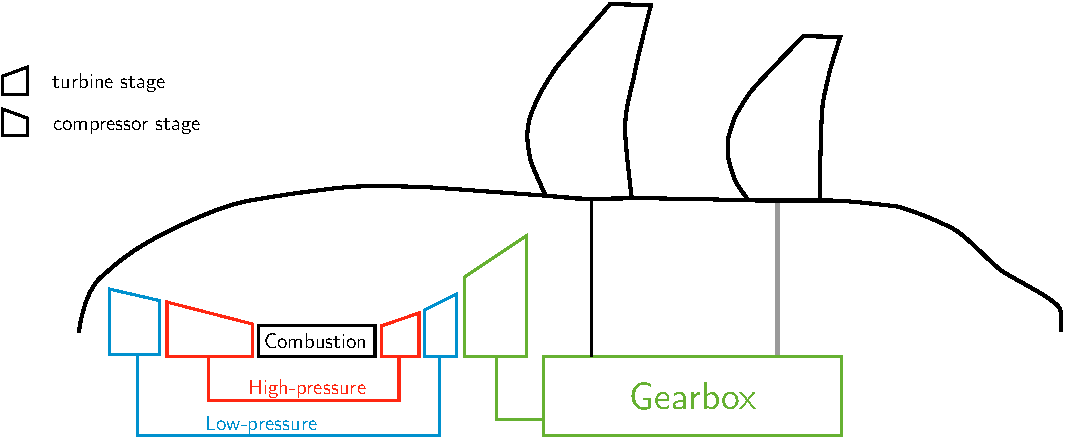
\includegraphics[width=.4\textwidth]{geared_cror.pdf}}
  \subfigure[Statorless low-pressure turbine design]{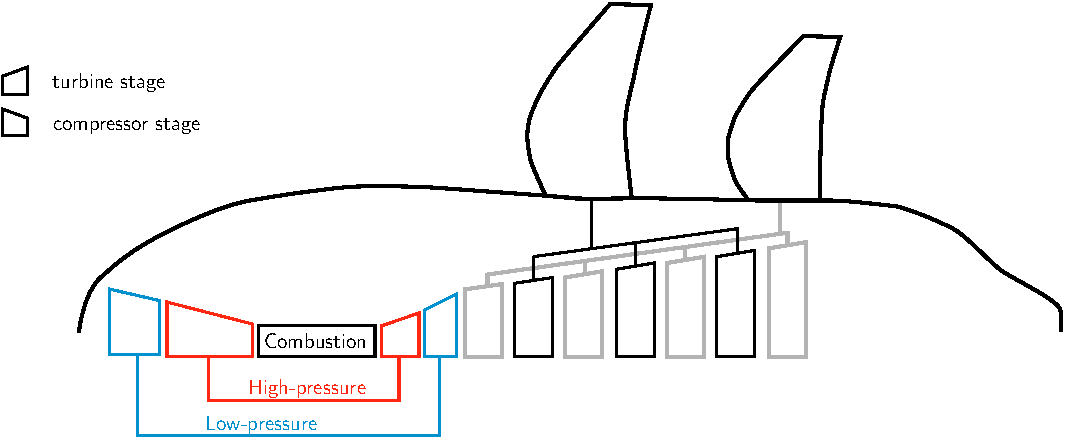
\includegraphics[width=.4\textwidth]{stator_less_cror.pdf}}
  \caption{Contra-rotating open rotor architectures.}
  \label{fig:cror_architectures}
\end{figure}

\subsection{Velocity triangle}
\label{sub:cror_velocity_triangle}

The basic idea behind the CROR concept is that a propeller has a 
better propulsive efficiency than a turbofan. The problem is that
a residual tangential velocity is present behind a propeller.
In fact, applying the velocity triangle to a propeller configuration
as shown in Fig.~\ref{fig:velocity_triangle_propeller}, one can
observe that the outlet velocity (noted $V^{out}_x$) is not axial
leading a tangential velocity $\Delta V_{\theta}$. This tangential forms
the swirl observe behind a propeller. First, this is a lost energy and
second, it produces a torque that has an impact on the flight dynamics
of the aircraft. To alleviate this effect, one can use two propellers
that are counter-rotating as for instance the TP$400$ propellers
in the Airbus-A$400$M military airplane but this does not recover
the swirl energy that is lost.

To do so, a second contra-rotating rotor can be used.
\begin{figure}[htbp]
  \centering
  \includegraphics*[scale=0.40]{velocity_triangle_cror.pdf}
  \caption{Velocity triangle applied to a contra-rotating open rotor configuration.}
  \label{fig:velocity_triangle_cror}
\end{figure}
Figure~\ref{fig:velocity_triangle_cror} shows the application
of the velocity triangle to a CROR configuration. The swirl
energy that was lost in the propeller is now used to 
produce more thrust. Thus, a CROR has a better propulsive
efficiency than a propeller.


\subsection{Similarity coefficients}
\label{sub:cror_similarity_coeff}

In the case of a CROR configuration, two rotors are considered.
Two main ways exists to evaluate the global value of the
similarity coefficients. The first one, chosen by
\citet{Bechet2011} among others, is to consider
that the non-dimensioning parameter $D$, $n$ and $J$ are those
of the front rotor for both rotors. 
The second one uses the non-dimensioning parameter of the current rotor,
as done by \citet{Stuermer2008} and \citet{Zachariadis2011}.
The traction and power coefficients of the rear rotor is
computed using its own advance ratio, diameter and rotation frequency.
Nevertheless, computing the advance ratio of the rear rotor, as
the free-stream velocity should be updated to take into account
for the acceleration generated by the front rotor. The free-stream
velocity is chosen to be $V_0$, which is of course not true.
The efficiency is computed rotor per rotor and then
assembled through an arithmetic summation. This is the approach retained
in this thesis.
